\articlehead{Our Fursonas Are Happier than We Are}{JM}{2012}

We furries, or at least most of us, have multiple identities.

Like everyone, we have our outward-facing human identity, named by our parents and constricted by whatever body it happens to be contained within. Our unique outward-facing identity is closely tied to our position in society and is tied to artificial constructs that crystallize our self into an acceptable bureaucratic package, such as our passports, our social security numbers, or our Google Plus accounts.

Furries usually also create one or more fictional identities. We name ourselves, select a combination of human and animal traits to create a new body, and often a new set of personality traits. Some furries, who create an avatar with interests (or physical dimensions) that do not easily gel with the real world, go further and create a fantasy universe.

Our furry identity is a personal creation, a kind of internal ghost accompanying the human that lurks around the real world. In situations where the real world is less intrusive, like corners of the internet or furry gatherings, our furry identities assert themselves and the human -- with its arbitrary name, body, and bureaucratic accoutrements -- is pushed to the background.

When the furry self is at the forefront, we experience the world in a different way. And, according to recently published data from the Anthropomorphic Research Project (based at the Niagara County Community College in the USA), we experience the world through the lens of an identity that is more mature, psychologically healthier, and happier than our human selves.

The ARP publishes results from two or three surveys each year. At this year's Furry Fiesta they performed psychological profiles and summarized the results against the well-regarded ``Big Five'' personality traits. Cleverly, they asked the furries to answer the questions twice: once for themselves and once for their fursona.

The biggest personality different between ‘human' and ‘furry' identity is also the most predictable: the fursonas are much more extroverted. This is due to the well-understood mask effect, a phenomenon familiar to anyone who has spent time on the inside of a fursuit.

The mask effect describes how people change their behaviour when behind a mask: they become less self-aware. The best-known experiment in psychological circles is a much-cited 2003 study that has the subject wear a mask, or stand in front of a mirror, and asks questions related to identity (ref). Participants wearing the mask demonstrate depersonalization and deindividuation.

More directly relevant to furries are studies on cosplayers. Researchers believe that people who attend sci-fi conventions in costume are undergoing ``self-administered mental health treatment''. (You can read more here on [adjective][species] here.)

The mask effect allows people who are normally reserved and risk-averse to trial outgoing and extroverted behaviour. While no studies have looked at furries specifically, the same behaviour can be observed in capering fursuiters. Psychologists believe that this helps shy people learn to feel more like their suited self: happy, generous, and more extroverted.

You can read more about research on cosplayers at the dedicated Psychology Today blog: http://www.psychologytoday.com/blog/the-superheroes.

The mask effect has other benefits beyond helping people overcome shyness: it can also help us mature. The reduction in self-awareness while wearing a mask (or fursuit) allows us to ‘advance scout' different personality traits. A fursuiter might, for example, act more flirtatious than the human inside would normally find comfortable, in a low-risk environment. This effect exists whether the mask is physical or virtual: we experience a similar drop in self-awareness when we socialize online in the guise of an alternate personality: our fursona.

Furries, through their fursona, experiment with many different personal traits. Most strikingly, many furries experiment with sexual identity or gender identity through their furry identity. For example, new furries joining the community notoriously tend to re-evaluate their sexual preference, starting heterosexual. There is strong evidence that this is true: data mining performed by [adjective][species] indicates that about half of heterosexual furries will change their sexual preference within their first five years in the community, usually to gay (Re-Evaluating Your Sexual Preference). We have no similar data for gender identity (numbers are too small for statistical analysis), however it is reasonable to assume that many transexuals experiment with a differently-gendered furry character as an important learning step toward eventual self-acceptance.

Aside from the mask effect, which explains why our fursonas are more extroverted than our human selves, the ARP data shows that our furry identities are different in other, more subtle ways.

The ARP data showing Big Five personality traits for furries (ref) is as follows:

\begin{figure}
  \begin{center}
    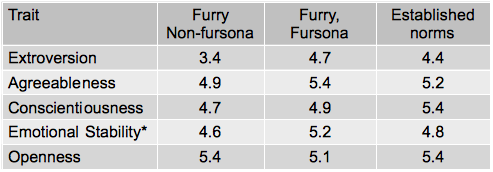
\includegraphics{content/assets/fursonas-happier--table}
  \end{center}
  \begin{caption}
    Personality traits

    * Minor note: emotional stability data is usually reported as Neuroticism in Big Five personality studies.
  \end{caption}
\end{figure}

This data suggests that, perhaps counter-intuitively, our fursonas are a normalizing influence on our personality. This is consistent with psychological theories on roleplaying, where people tend to create a fictional identity that is a positive rolemodel for themselves. This theory, key to some cognitive behavioural therapy methodologies, is usually applied to children roleplaying but also applies to superhero cosplay, and -- it seems -- to furries as well.

The ARP data also shows that the differences between our human and furry selves are similar to the differences between college age and middle adulthood. That is, our furry selves are also more mature.

\begin{figure}
  \begin{center}
    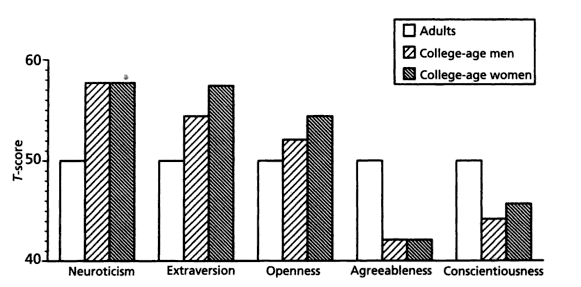
\includegraphics{content/assets/fursonas-happier--bar-chart}
  \end{center}
  \caption{Ref Costa \& McRae 1992}
\end{figure}

There is some logic to this. Data shows that personality is in flux until about age 30. Furries are a young group, with a median age of 22 (ref) so collectively, our personalities are still developing.

Changes in personality during maturation occur largely as we become more self-accepting and less self-centred. It makes sense that our imaginary furry selves are less focussed on our own imperfections.

Personality changes as we age into 30-plus adulthood are also correlated with increased happiness and contentment (ref). There is a large body of research on the topic which shows that, as we mature, we learn to trust ourselves and empathize with other people. Between college age and middle adulthood (30-plus again) this translates into \textit{``increased well-being''} (Mortimer 1928), \textit{``decreased alienation and social criticism''} (Jessor 1983), as we become \textit{``less emotional and better socialized''} (Hann 1986).

Our fursonas display many of these traits. They are forging a path of self-improvement: from them, we become more mature, less divergent from others around us, and -- most importantly -- happier.

The ARP's website is here -- https://sites.google.com/site/anthropomorphicresearch/home. Their most recent publication is a comprehensive analysis of data collected at Anthrocon 2012.

There are two ways in which life can improve: through a change in the outside world, or through personal change. As we mature, we become less self-centred, making it easier for us to self-analyse in a balanced fashion. As we explore our own personalities through our furry identity, we can learn to effect positive change.

It is a sign of maturity to look internally for ways to improve one's life. We have control over our own actions and our interpretation of the world around us: we do not have control over much of the external world or the people in it.

To put it another way: when exposed to an enraging YouTube comment thread, we can either ignore the comments or engage with them. The more mature approach is to ignore the comments, which brings an immediate increase in happiness as we focus on something else. It is less mature (albeit completely normal) to try to correct the behaviour of the other commenters -- as we all know, this is a dark path to frustration and unhappiness.

For another example, I have been exposed recently to a few articles and comic strips titled ``How To Treat Your Introvert'' (or similar). It's usually linked by someone who considers themselves to be introverted, in the hope that people will read this advice and accordingly treat them with a greater understanding.

(Language note: this use of the term ``introvert'' is slightly different from that used by psychologists. It doesn't easily relate to extroversion as a Big Five personality trait.)

\begin{figure}
  \begin{center}
    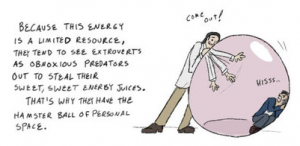
\includegraphics{content/assets/fursonas-happier--bubble}
  \end{center}
  \caption{Ref Sveidt on DeviantArt}
\end{figure}

\begin{figure}
  \begin{center}
    
\includegraphics{content/assets/fursonas-happier--introverts}
  \end{center}
  \caption{Ref questionablylate.tumblr.com}
\end{figure}

In extremis, such advice depicts a pathologically shy person being harassed by a sociopath. This purports to represent the plight of the intovert: they feel victimized by the outside world, preferring to exist largely inside the safety of their own head.

The advice is doubly misleading. Firstly, everyone feels victimized by the outside world. We all find socializing stressful, and we are all haunted by memories of humiliating social experiences. The advice seems profound because everyone feels that way at least some of the time -- horoscopes are designed to work in the same way. Secondly, the advice implies that introversion is innate; a fixed aspect of personality. It's not.

It's also terrible advice. The intent and spirit of the advice is good -- it suggests ways in which we can care for people around us. It's bad advice because the reader is supposed to identify with the introvert, the person portrayed as a powerless victim of the world around them. (Nobody identifies with sociopaths, not even actual sociopaths.) To hope that the world will change to meet the needs of our introvert is to hope to improve the discourse on a YouTube comments thread through sensible diplomacy.

People who feel introverted can improve their life by looking inwards, and considering things they can control. This is the more mature approach.

A better set of advice might be:

\begin{itemize}
  \item Be empathetic. Spend more time listening to other people; they will relax if they feel their own social needs are being met.
  \item Socialize online via your fursona. You will feel less self-conscious.
  \item Stop hanging around with sociopaths.
\end{itemize}

Looking inwards to effect change will help our introvert find social experiences that are happy, rather than stressful. After all, that's what our fursonas do.

Finding contentment in this world is an endless and difficult task. Happily, we can expect to improve as we mature. Even better, we furries have a happy, healthy rolemodel -- our animal-person alter-ego -- who can lead the way.

Just ask yourself: \textit{What Would a Furry Do?}
